\documentclass{loyola-beamer}
\renewcommand{\titlelogo}{logo/luc-rev.svg}
\renewcommand{\slidelogo}{logo/luc.svg}
\usepackage{physics}
\usepackage{graphicx}
\usepackage{hyperref}


\title{Coherent States}
% \subtitle{Made with Beamer}
\author{Alfaifi, Ammar}
\institute{KFUPM}
\renewcommand{\slidefoot}{Department of Physics - PHYS410}

\begin{document}

\begin{titleframe}{}
	\maketitle
\end{titleframe}

\begin{frame}{Contents}
	\tableofcontents
\end{frame}


% Start of the slides

\begin{titleframe}{Comparison}
	Stationary States vs. Coherent States
\end{titleframe}

\section{Stationary States}

\begin{frame}{Stationary States}
	Stationary states are eigenstates of the Hamiltonian $\hat{H}$

	\vspace{\baselineskip}
	For quantum harmonic oscillator the Hamiltonian is

	\begin{align*}
		\hat{H} = \hbar \omega \left(  a^\dagger a + \frac{1}{2} \right)
		\label{eq:Hamiltonian}
	\end{align*}

	\begin{align*}
		\hat{H} |n \rangle = E_n |n \rangle
	\end{align*}

	\begin{align*}
		\hat{a} |n \rangle = \sqrt{n} |{n-1} \rangle
	\end{align*}

\end{frame}


% New slide
\section{Coherent States}

\begin{frame}{Coherent States}
	Mathematically, a coherent state is defined to be the (unique)
	eigenstates of the annihilation operator â with corresponding eigenvalue $\alpha$.

	\vspace{\baselineskip}
\end{frame}


\begin{frame}{What are Coherent States?}

	Coherent states are defined as eigenstates of the annihilation operator. Specifically, they are defined as:
	\begin{equation}
		\hat{a} \left| \alpha \right\rangle = \alpha \left| \alpha \right\rangle
	\end{equation}
	since $\hat{a}$ is not hermitian, $\alpha$ is a complex number and $\left|\alpha\right\rangle$ is the coherent state.

\end{frame}

\begin{frame}{Derive Coherent States}

	We write the coherent states in the basis of the Hamiltonian.

	\begin{align*}
		| \alpha \rangle  = \sum_{n=0}^{\infty} \, c_n(\alpha) |n \rangle;
		\qquad c_n(\alpha) = \bra{n} \ket{\alpha}
	\end{align*}

	\begin{align*}
		\hat{a} \ket{\alpha} & = \sum_{n=0}^\infty c_n(\alpha)\, \hat{a} \ket{n}
		= \sum_{n=1}^\infty c_n(\alpha)\sqrt{n}\, \ket{n-1}                            \\
		                     & = \sum_{n=0}^\infty c_{n+1}(\alpha)\sqrt{n+1}\, \ket{n}
	\end{align*}

	\begin{align*}
		\hat{a} \ket{\alpha} = \alpha \ket{\alpha} \Rightarrow
		\sum_{n=0}^\infty c_{n+1}(\alpha)\sqrt{n+1}\, \ket{n}
		= \alpha \sum_{n=0}^\infty c_{n}(\alpha)\, \ket{n}
	\end{align*}

\end{frame}

\begin{frame}{Derive Coherent States}
	\begin{align*}
		c_n(\alpha) = \frac{\alpha^n}{\sqrt{n!}}\, c_0
	\end{align*}

	The coherent states are
	\begin{align*}
		\ket{\alpha} = \sum_{n=0}^\infty \frac{\alpha^n}{\sqrt{n!}} c_0(\alpha) \, \ket{n}
	\end{align*}

	Normalization
	\begin{align*}
		1= \bra{\alpha}\ket{\alpha} & = | c_0(\alpha) |^2
		\overbrace{\sum_{n=0}^\infty \frac{|\alpha|^{2n}}{n!}}^{e^{|\alpha|^2}} \\
		| c_0(\alpha) |^2           & = e^{-|\alpha|^2}
		\Rightarrow c_0(\alpha) = e^{-|\alpha|^2/2}
	\end{align*}



\end{frame}

\begin{frame}{Derive Coherent States}
	Finally, the coherent state in the energy basis is
	\begin{align*}
		\ket{\alpha} = e^{-|\alpha|^2/2}\,
		\sum_{n=0}^\infty \frac{\alpha^n}{\sqrt{n!}} \, \ket{n}
	\end{align*}

\end{frame}

\begin{frame}{Properties of Coherent States}

	Coherent states have several important properties which make them useful for many applications.

	\begin{itemize}
		\item Coherent states are minimum-uncertainty states: they have the minimum possible uncertainty in both position and momentum.
		\item Coherent states have a Gaussian wavefunction, which makes them easy to work with.
		\item Coherent states are stable: they remain unchanged over time.
		\item Coherent states can be used to approximate classical behavior.
	\end{itemize}

\end{frame}

\begin{frame}{Applications of Coherent States}

	\begin{itemize}
		\item coherent states are used in quantum optics to describe light.
		\item coherent states can be used to simulate the behavior of classical systems.
		\item coherent states can be used to encode quantum information.
		\item coherent states are used in quantum computing to implement quantum algorithms.
	\end{itemize}

\end{frame}

\section{Time Evolution}

\begin{frame}{Time Evolution}
	\begin{align*}
		\ket{\psi(0)} = \ket{\alpha_0} = e^{-|\alpha_0|^2/2}\,
		\sum_{n=0}^\infty \frac{\alpha_0^n}{\sqrt{n!}} \, \ket{n}
	\end{align*}

	\begin{block}{Harmonic oscillator}
		$\hat{H}$ is time independent: conservative system.
	\end{block}


	\begin{align*}
		\ket{\psi(t)} = e^{-|\alpha_0|^2/2}\,
		\sum_{n=0}^\infty \frac{\alpha_0^n}{\sqrt{n!}} \,  e^{-iE_nt\hbar} \ket{n}
	\end{align*}
\end{frame}

\begin{frame}{Time Evolution}
	\begin{align*}
		\ket{\psi(t)} e^{-i\omega t/2} e^{-|\alpha_0|^2 /2}
		\sum_{n=0}^\infty \frac{(\alpha_0 e^{-i\omega t})^n}{\sqrt{n!}}\, \ket{n}
	\end{align*}
	let $\alpha \equiv \alpha_0 e^{-i\omega t}$

	\begin{align*}
		\ket{\psi(0)} = \ket{\alpha_0} \rightarrow \ket{\psi(t)} = e^{-i\omega t/2} \ket{\alpha};
	\end{align*}

	\begin{block}{Conclusion}
		A coherent state stays coherent at all times.
	\end{block}
\end{frame}


\begin{frame}{Time Evolution}
	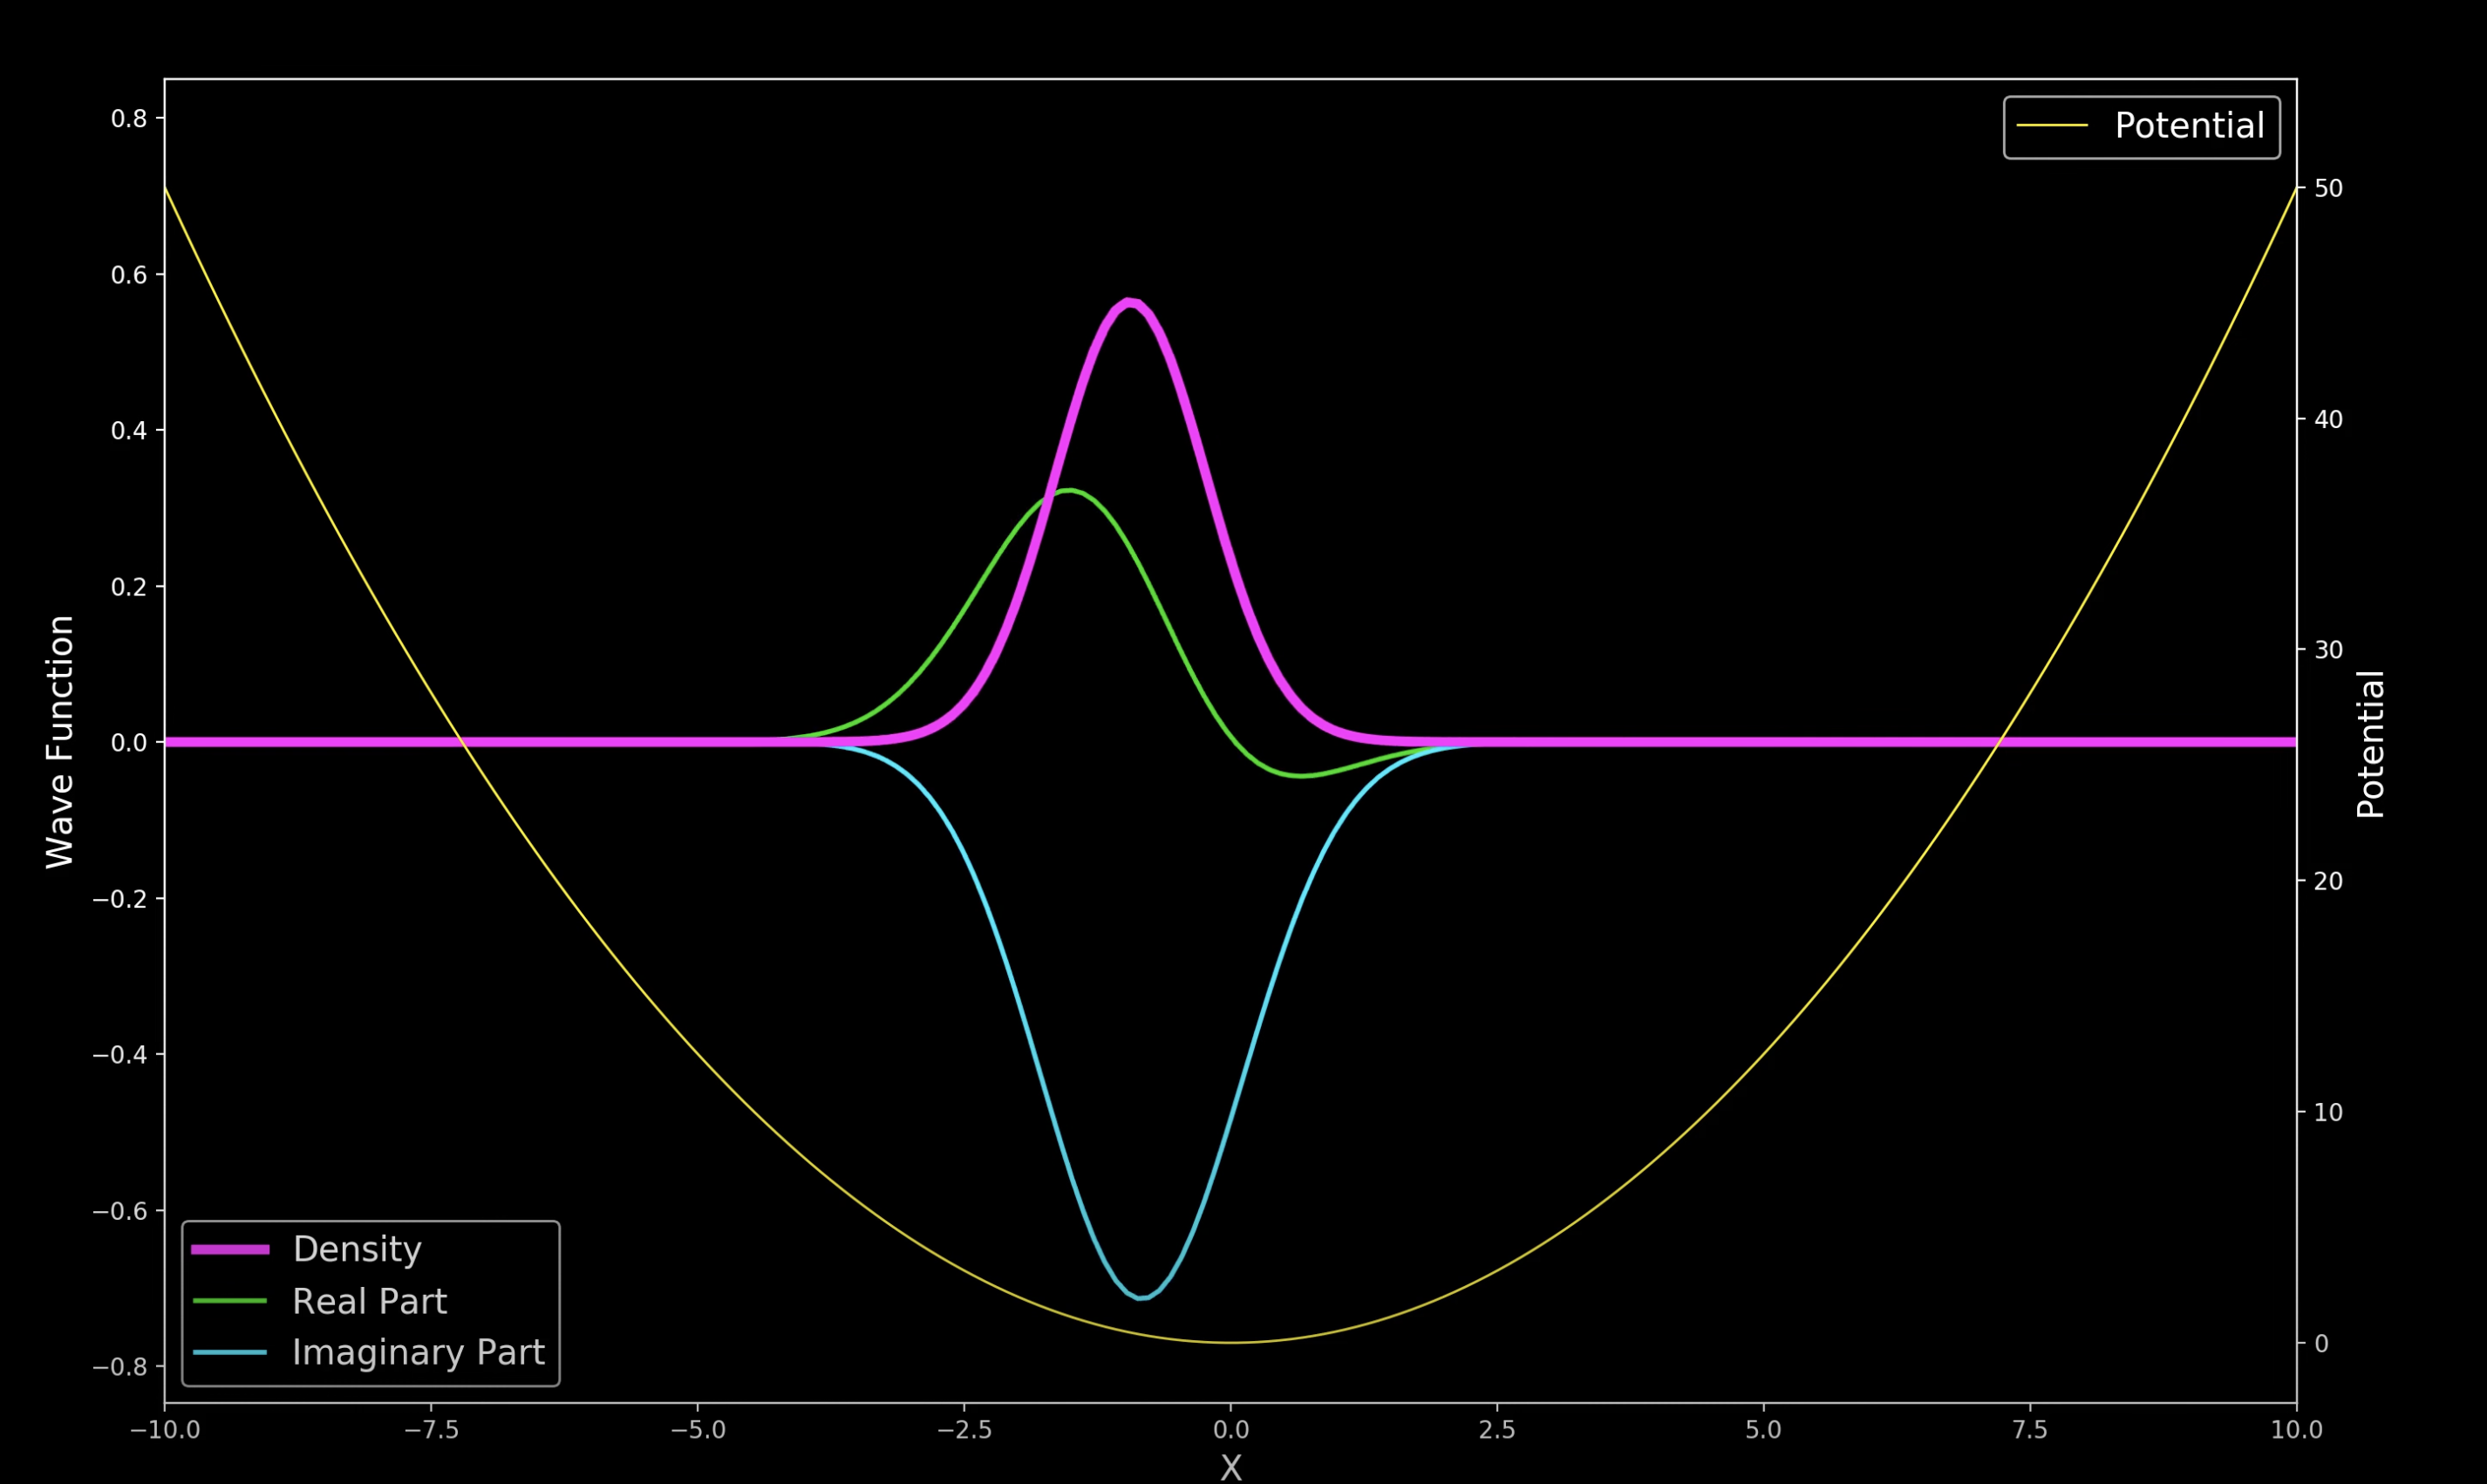
\includegraphics[width=0.9\textwidth]{anim.png}

	\href{https://www.youtube.com/watch?v=60OD3fahkHU}{https://www.youtube.com/watch?v=60OD3fahkHU}
\end{frame}

\section{Creation Operator}

\begin{frame}{About Creation Opreator}
	\begin{alertblock}{Note}
		Creation operator has no eigenstates.
	\end{alertblock}
	\begin{align*}
		\hat{a}^\dagger \ket{\lambda} = \lambda \ket{\lambda}
	\end{align*}
	\begin{align*}
		\sum_{n=0}^\infty c_n \sqrt{n+1}\, \ket{n+1}
		= \lambda \sum_{n=0}^\infty c_n\, \ket{n}
	\end{align*}
	\begin{align*}
		\ket{0} & : \quad 0 = \lambda c_0 \Rightarrow c_0 =0               \\
		\ket{1} & : \quad c_0 = \lambda c_0 \Rightarrow c_1 =0             \\
		        & \vdots                                                   \\
		\ket{n} & : \quad c_{n-1} \sqrt{n}=\lambda c_n \Rightarrow c_n = 0
	\end{align*}

\end{frame}

\begin{frame}{Conclusion}

	In conclusion, coherent states are special types of quantum states which have several
	useful properties and applications. They are widely used in quantum physics, quantum optics,
	and quantum information.

\end{frame}





\begin{titleframe}{Thank you for listening!}

\end{titleframe}

\end{document}
